\cleardoublepage
\chapter{Related Work}
\label{ch:relatedwork}
\label{ch:chapter2}

\section{Long-Context LLMs}

Memory mechanisms have long been studied in Natural Language Processing for modeling long-term dependencies. Before the introduction of the transformer architecture, Recurrent Neural Networks (RNNs) represented the state-of-the-art language models. RNNs incorporate a recurrence mechanism in which each hidden state retains important information about the input sequence up to that point, allowing it to serve as context for subsequent parts of the input \cite{alma991005389998907681}. However, these models were not only prohibitively expensive to train due to their recurrence mechanisms but also difficult to optimize due to issues like vanishing and exploding gradients \cite{dai-etal-2019-transformer}. The introduction of the self-attention mechanism in transformers marked a significant breakthrough \cite{10.5555/3295222.3295349}. However, a key limitation of transformers is their reliance on a fixed context window, which constrains their ability to model long-term dependencies. Some recent architectures have attempted to introduce recurrence into the transformer architecture, but these remain prone to information loss \cite{dai-etal-2019-transformer}. Other approaches focus on positional interpolation which rescales position indices to match those used during the pre-training, though they are only suitable for RoPE-based LLMs, and more importantly the extent to which the context window can be extended is still limited \cite{chen2023extendingcontextwindowlarge}\cite{ding2024longrope}. \\

\noindent Wang et al. proposed a model architecture that incorporates a residual side network, which serves as long-term memory storage for the LLM \cite{wang2023augmentinglanguagemodelslongterm}.\\

\noindent While this area of research is promising, using the context window for memory management alone comes with significant challenges. One major limitation is the high costs associated with embedding all memories directly into the context window as it leads to increased token usage, and blurs the separation between the different types of memory. Moreover, this approach makes it harder for the model to effectively attend to the most relevant information in the context, a problem that has previously been observed in long-context LLMs \cite{liu2023lostmiddlelanguagemodels}.

\section{Retrieval Augmented Generation}

Retrieval Augmented Generation enhances LLMs by integrating relevant knowledge from external data sources into their context \cite{lewis2021retrievalaugmentedgenerationknowledgeintensivenlp}. This strategy has been expanded to implement long-term memory for LLM conversational agents by allowing the agent to also write to external sources \cite{Zhong_Guo_Gao_Ye_Wang_2024}. \\ 

\noindent Various studies have explored different retrieval granularities, including chunks, summaries, and knowledge triples \cite{zeng2024structuralmemoryllmagents}, as well as different retrieval algorithms such as BM25 and semantic similarity.\\

\noindent Graph RAG extends this approach by using an LLM to extract entities and relationships from a corpus, constructing a knowledge graph that enables more effective reasoning over the data. This structured representation helps answer global questions where conventional RAG methods often underperform \cite{edge2024localglobalgraphrag}. HippoRAG is a recent novel system that also leverages a graph and presents an analogy with neurobiological systems \cite{NEURIPS2024_6ddc001d}.\\

\noindent Unfortunately, RAG alone has been shown to be inefficient for solving tasks that require more reasoning capabilities such as MHQA, and more complex systems are required to implement long-term memory that can be integrated seamlessly with reasoning steps.

\section{Prompting Methods}

Numerous prompting methods have been developed to exploit the capabilities of LLMs, enabling them to reason over intricate datasets. Techniques such as Chain of thought (CoT) and few-shot prompting have demonstrated impressive results in tackling complex tasks, including mathematical reasoning \cite{wei2023chainofthoughtpromptingelicitsreasoning}. Other prompting methods seek to exploit the reasoning capabilites of LLMs. ReAct is a prompting framework designed to interleave reasoning and action, and is widely used in language agents to aid them in decision-making \cite{yao2023react}. In particular, for long-inputs, \textit{PEARL} (\textbf{P}lanning with \textbf{E}xecutable Actions for \textbf{R}easoning over \textbf{L}ong documents) is a prompting method which consists of three stages. First, an LLM is prompted to generate a list of actions that could help answer a question about the document. Second, the LLM formulates a plan that outlines the execution of actions from the previous step. Finally, the LLM executes the plan to generate the final answer. This approach uses the output of each action to inform the next step, ultimately guiding the model to generate a correct answer \cite{sun-etal-2024-pearl}. Similarly, Yue et al. proposed \textit{Iterative Demonstration-Based RAG}, a method designed to handle complex queries by decomposing them into simpler sub-queries. RAG is then applied to each subquery, leading to improved performance over conventional RAG \cite{yue2024inferencescalinglongcontextretrieval}.

\section{Language Agents}

Language Agents refer to agents that integrate LLMs for reasoning and communication, using language as their primary means of interaction with the environment and decision-making \cite{language-agent-tutorial}. One of the core aspects of agents is memory, which can be viewed as an internal mechanism that enables them to update their long-term memory, and retrieve past memories. MemGPT and Graph Reader are examples of language agents that incorporate these concepts where each one operates within a distinct environment \cite{packer2024memgptllmsoperatingsystems}\cite{li2024graphreaderbuildinggraphbasedagent}.\\

\noindent Memory, as understood in cognitive systems and inspired by human long-term memory, is threefold. Episodic memory stores experiences, semantic memory stores knowledge or facts, and procedural memory stores skills \cite{sumers2024cognitive}. AriGraph is a language agent that integrates episodic and semantic memories in a knowledge graph, allowing the agent to access and utilize this structured information for reasoning \cite{anokhin2024arigraphlearningknowledgegraph}.

\begin{figure}
    \centering
    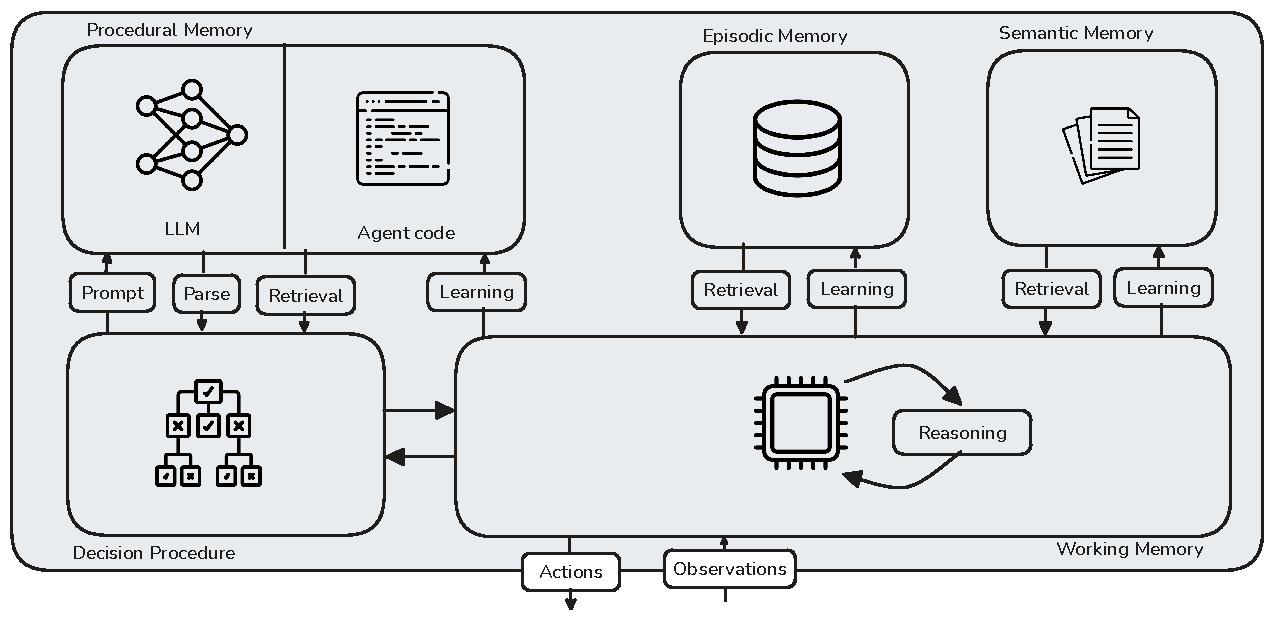
\includegraphics[width=0.95\textwidth]{images/cognitive-arch.pdf}\\[-0.25cm]
    \caption{Cognitive architectures for language agents \cite{sumers2024cognitive}.}
    \label{fig:cognitive-arch}
\end{figure}
